% !TEX root = ../my-thesis.tex
%

\chapter{Implementation}
\label{sec:implementation}

\begin{figure}[htb]
	\centering
	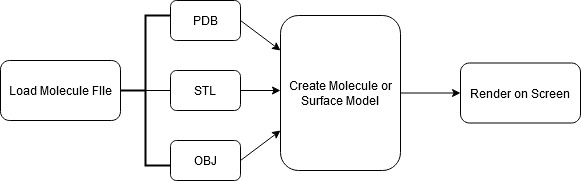
\includegraphics[width=\textwidth]{gfx/visualisation_pipeline.jpg}
	\caption{Visualisation Pipeline.}
	\label{sec:implementation:vispipe}
\end{figure}

Figure \ref{sec:implementation:vispipe} shows the general visualisation pipeline of the \textit{Molecule Visualizer}. After selecting a new molecule to display the \textit{loadFile()} event is responsible for determining which \textit{Molecule Representation} was used and extracting the file's content. The structure of the extracted content depends on the representation used and the corresponding loader provided by three.js. According to the information provided by the loaders the molecule model is generated and rendered afterwards. The following sections will detail the process of visualisation and describe the different molecule models and molecule representations supported by the \textit{Molecule Visualizer}. Before that we will outline the structure of our project and how the different classes are connected. Furthermore the communication between the Graphical User Interface (GUI) and the Visualizer is going to be discussed. Currently, they communicate with each other via the use of events which are managed by a global instance of the \textit{EventManager} class. Lastly, the use and application of VR in our application will be explored. We decided to only include minimal interaction possibilities during the VR session and no GUI for changing the displayed molecule or its representation. Here we will explain our reasoning as to why we did this.

\section{Overview}
\label{sec:implementation:overview}

In order to create our visualisation application we decided to follow an object-oriented approach. Reason for that is the goal of designing a tool that can easily be extended and has interchangeable components. This has the advantage that one can create new objects that inherit from our classes and add new functionalities without much effort. We also managed to minimise dependencies between objects by grouping together functions that perform similar tasks, i.e. all visualisation-related functions belong to one class, all GUI-related functions belong to a class etc. If two classes need to communicate with each other this can be achieved by either storing an instance of the object in question or by using event-based communication. We preferred to use Event communication as often as we could, because it helps decoupling objects and prevent unnecessary dependencies.

\begin{listing}[H]
\begin{minted}[autogobble, bgcolor=bg, breaklines, linenos]{javascript}
// Constant section.
const NEAR = 1e-6;
const FAR = 2000;
const scene = new THREE.Scene();
const camera = new THREE.PerspectiveCamera(50, innerWidth / innerHeight, NEAR, FAR);
const container = document.getElementById('container');
const renderer = new THREE.WebGLRenderer({canvas: container, antialias: true, logarithmicDepthBuffer: true});
const stats = new Stats();
const cameraGroup = new THREE.Group();
const prevGamePads = new Map();
let cameraVector = new THREE.Vector3();
let speedFactor = [0.1, 0.1, 0.1, 0.1];
let frontLight1, frontLight2, backLight1, backLight2;
// Properties section.
class Visualizer {
	constructor() {
		this.root = new THREE.Group();
		this.controls = new TrackballControls(camera, renderer.domElement);
		this.objectPicker = new ObjectPicker(this.root, camera);
		this.moleculeModel = new Model();
		this.renderRequested = false;
		this.debugGUI = new VisualizerGUI();
		this.moleculestruct = {};
		this.modal = new Modal(document.querySelector('#modal'));
		this.changedAtomColor = new Map();
	}
}	
\end{minted}
\caption{Structure of the \textit{Visualizer} class.}
\label{sec:implementation:overview:visualizer}
\end{listing}

The \textit{Visualizer} class contains the main functionality of our tool. Each of the other classes is connected to it via Event-based communication to trigger changes in the visualisation. Code snippet \ref{sec:implementation:overview:visualizer} shows the general structure of \textit{Visualizer}. The class has references to the other classes in order to create event functions that should be triggered once the corresponding functionality has been triggered. As the \textit{Visualizer} acts as the main part of our application it also keeps references to render-related objects like \textit{scene}, \textit{camera} or \textit{renderer}. Rendering has been realised using render-on-demand which means that we only want to render when something about the representation of the molecule changed like the model or atom colors. This increases the performance of the application and saves resources by calling the render routine only when necessary. During rendering we use a special kind of meshes to increase performance called \textit{InstancedMesh}. They work just like normal mesh objects in three.js, but they also require an \textit{instanceCount} parameter that specifies how many instances of this mesh should be rendered. That means you can render multiple objects in one render call. As previously mentioned, the \textit{Visualizer} also sets up the Event functions that should be called when their associated functionality is triggered. For example changing the rendered molecule if you chose a new file via the GUI. This is done by first defining the Event function and then registering it in the \textit{EventManager} class by calling \textit{EventManager.addEvents}.

\begin{listing}[H]
\begin{minted}[autogobble, bgcolor=bg, breaklines, linenos]{javascript}
// Properties section.
class EventManager extends EventDispatcher {
	constructor() {
		this.managedEvents = new Map();
	}
}

// Example of how to add event listeners to objects.
EventManager.addEvents(object, [event1, event2, ...], [eventFunction1, eventFunction2, ...]);

// This is how objects and events are stored internally.
{object: {event1: eventFunction1,
          event2: eventFunction2,
          ...},
}
\end{minted}
\caption{Structure and usage example of the \textit{EventManager} class. In order to add event listeners to objects you have to provide a reference to the object, a list of events and a list of corresponding event functions. Note that event and function have to have the same position in their respective arrays in order to store them correctly.}
\label{sec:implementation:overview:eventmanager}
\end{listing}

In order for our classes to communicate with each other we created the \textit{EventManager} class. This class is responsible for managing events and the corresponding listener objects. This way we are able to freely add and remove events any time necessary. Code snippet \ref{sec:implementation:overview:eventmanager} shows the structure of the \textit{EventManager} and an example of how to use the object. You are able to add multiple events to an object by calling \textit{EventManager.addEvents}. In order to manage the objects we store them inside a map with the object being the key and the value being another object containing the added events and their corresponding functions. The structure of the map is also illustrated in code snippet \ref{sec:implementation:overview:eventmanager}.

The \textit{ObjectPicker} class is responsible for interacting with the rendered molecules in the normal scene as well as in the VR environment. A raycaster is used to cast a ray from the mouse position and detect if you clicked an atom or not. Clicking atoms informs the \textit{Visualizer} class to show a modal containing information about the atom like its position or color. Inside the VR scene a ray is cast from the controller's position instead and checked for intersections with atoms.

\begin{listing}[H]
\begin{minted}[autogobble, bgcolor=bg, breaklines, linenos]{javascript}
// Create GUI structure.
const api = {
	button: () => {	// Buttons are defined via callbacks.
		...
	},
	checkbox: false	// Checkboxes are defined via booleans.
	dropdown: {	// Drop-down menus are defined by listing the options within an object.
		...
	},
	color: 0x00Ff00,	// Colors are defined by using their hexadecimal representation.
	input: '',	// Input fields are defined by using a string literal.
	
	// Create GUI folder where gui is the GUI to add the folder to.
	const folder = gui.addFolder('folder');
	// Add GUI element to folder. In this case we add a button to the GUI.
	folder.add(api, 'button');
};
\end{minted}
\caption{Example of how to define and bind GUI elements.}
\label{sec:implementation:overview:visualizergui}
\end{listing}

Our GUI is defined inside the \textit{VisualizerGUI} class. It is closely connected to the \textit{Visualizer} class by sending events every time a setting has been changed. We inherited from the GUI class of three.js to generate the interface and manage our settings. The GUI consists of folders in which you can add elements like buttons or checkboxes. Code snippet \ref{sec:implementation:overview:visualizergui} illustrates the process of adding elements to the GUI. First you create the structure of the GUI as a JavaScript object. Depending on the content of its entries the added elements will differ, e.g. buttons are defined as functions inside the structure object. Then you create a folder for the GUI and add the element to it by referencing the structure object and the corresponding field name.

Showing atom information after clicking them is handled by the \textit{Modal} class. It receives a reference to an HTML element that should act as the modal body and will be populated by the \textit{Modal} class. After an atom has been clicked the content of the modal window will be constructed and then set via the \textit{Modal.setModalContent} method. Closing the modal can be done by clicking on its close button or clicking anywhere on the browser window. Currently modals are only available after loading molecules from Protein Data Bank (PDB) files as they provide atom information like periodic table symbol or color after parsing them. 

The \textit{Model} class handles management of the currently chosen molecule model and the corresponding mesh(es). It is also responsible for creating them in the first place. After loading a molecule or choosing another representation the \textit{Model} class is tasked with (re-)rendering the molecule according to the chosen representation. 

\section{Molecule Representation}
\label{sec:implementation:molrepr}

The first part of the visualisation pipeline is determining which type of molecule file is loaded and extracting its contents. Each file type stores various pieces of information regarding the molecule's composition and structures them differently. Currently, our Molecule Visualizer supports three different formats of molecule files: PDB, Wavefront .obj \cite{article} (OBJ) and Stereo Lithography \cite{BibEntry2019Sep} (STL). While PDB files only store the position of the atoms within the molecule OBJ and STL files store the coordinates of all vertices and faces that form the mesh. In the following two sections we are going to discuss the properties of the previously mentioned file formats as well as their advantages and disadvantages. Lastly, we will elaborate on their use case and how such files are handled within our application.

\subsection{Standard Representation}
\label{sec:implementation:molrepr:pdb}

The PDB file format is used for describing the structure of molecules that are included in the Protein Data Bank. It is a text-based format which contains information regarding nucleic acids within the molecule, atom positions and their connectivity as well as secondary structures \cite{BibEntry2022Jan}. PDB files have a width limit of 80 columns which stems from its introduction in 1970s. During that time punch cards were used to store data in a portable format and cards with 80 columns were the most commonly used ones \cite{Maxfield2011Oct}. Each line has to start with a specific keyword indicating what type of content to expect e.g. atomic coordinates or information regarding the nucleic acids present.

The most important keywords for our application to be able to render the described molecules are ATOM and CONECT as three.js already provides a loader called \textit{PDBLoader} that is capable of parsing PDB files. With the help of those tags the \textit{PDBLoader} constructs a JSON object which contains three fields: \textit{atomPositions}, \textit{bondPositions} and \textit{json}. The first two entries are \textit{BufferGeometries} that hold the positions of the atoms and bonds (in case of \textit{atomPositions} the atom colors as well). \textit{json} contains atom meta-data regarding position, color and periodic table symbol. This information is displayed inside modals which are triggered after clicking an atom. 

PDB files contain not only information about the basic geometry of the molecule, but also about its Secondary Structures. Secondary Structures occur based on the conformation of the atoms within a protein and are essential for defining a protein's structure \cite{DEGREVE2014384, 10.3389/fbioe.2021.687426}. The two most common types are $\beta$-Sheets and $\alpha$-Helices. In order to visualise those structures it is necessary to know which amino acids take part in forming the $\beta$-Sheets or $\alpha$-Helices which is exactly what PDB files provide. A different loader would be required as the one provided by three.js only parses the ATOM, HETATOM or CONECT lines in the files. This would mean that either the \textit{PDBLoader} has to be extended or another parsing library for PDB files has to be used. As one of our future goals is to integrate the \textit{Molecule Visualizer} into BALL.jl where we leave the molecule file handling to the Julia backend we deemed it not necessary to extend the \textit{PDBLoader} or use an external parser. Furthermore, the use of an external tool would require us to create the \textit{BufferGeometries} for atoms and bonds ourselves while this is already handled by three.js' loader. 

\subsection{Surface Representation}
\label{sec:implementation:molrepr:surface}

PDB files describe molecules in terms of atom positions and which atoms are bonded whereas STL and OBJ files represent their surface as a surface mesh. The surface mesh offers a clearer understanding of a molecule's three-dimensional structure and is also vital for simulations in which you try to dock smaller compounds onto proteins. STL files encode objects as a tessellated two-dimensional surface, i.e. a triangle mesh approximating the objects' surface \cite{SZILVSINAGY2003945}. For each triangle the following information is stored: its normal and the vertex coordinates. There is no information held regarding material or color of the object.

STL files with the \textit{solid} keyword followed by the name of the object. Triangles are stored by first declaring their normal, then each vertex by its coordinates within the mesh. Coordinates have to be represented as floating point numbers following the format sign-mantissa-\textit{e}-exponent. After all triangles have been defined the file ends with the \textit{endsolid} keyword. To ensure the file's validity it has to follow specific rules \cite{HAMANN1994197}. These rules ensure that the content of the STL file is valid and a correct tessellation of the object's surface. In order for the mesh to be connected each triangle should share at least one Vertex with other triangles. To prevent bifurcations an edge should only be shared by at most two triangles. 

OBJ files are able to represent the surface of an object as well. Similar to STL files they save information about the surface mesh by using the vertex coordinates and triangle faces. Additionally, vertex normals are stored as well which enables the use of Smooth Shading techniques such as \textit{Phong Shading}. As a result the rendered surface has a more natural appearance than surfaces generated from STL files. There is also a difference in how face normals are handled. While they are explicitly given for STL models, in OBJ they are inferred from the vertex coordinates as they are given in counter-clockwise order by default \cite{Iqbal2019Sep}.

One major advantage of OBJ files over STL is the realistic appearance of objects due to Smooth Shading and more accurate representation. Curved surfaces also cannot be precisely rendered using triangle meshes which means a loss in accuracy. A solution would be to use more triangles to approximate the curve, but this would result in extremely large STL files. To circumvent this problem, OBJ files are able to leverage techniques such as free-form geometry or surfaces \cite{Iqbal2019Sep}. 

\section{Molecule Models}
\label{sec:implementation:molmodels}

After identifying the type of representation used in the molecule file and parsing its content the actual model has to be created. Depending on the representation the Molecule Visualizer provides various model options to choose from. In total three molecule models are supported: Ball and Sticks, Wireframe and Space-Filling (Van der Waals. Those models are only available after loading a PDB file as STL and OBJ files only provide information for the molecule surface but not about the individual atoms or bonds. Each model presents different advantages regarding molecule properties, e.g. geometry, size, structure and interaction of molecules. We are going to give a short introduction to the models and their purpose in molecule visualization followed by an explanation on how they are implemented in our application.

\subsection{Ball and Stick}
\label{sec:implementation:molmodels:ballstick}

The Ball and Stick model is one of the basic visualisation models for chemical compounds and molecules. Atoms are represented by coloured spheres and bonds as small sticks. This representation is useful for examining the bonds of a molecule as they are explicitly shown and represented with their correct angles. One downside to the model is that it cannot accurately show the relative space covered by the molecule as the bond length compared to the radii of the atoms is made to be longer \cite{Hamzah2022Jul}. The bonds are more visible this way and the model is more simplified at the cost of an exact spacial representation. As such, Ball and Stick models are useful when it comes to analysing atomic bonds and the geometry of larger biological molecules.

We realized the Ball and Stick model in our application with the use of \textit{InstancedMeshes}. As the atoms and bonds only differ in color and scaling we could leverage the ability of \textit{InstanceMeshes} to create multiple objects at once with a single call to the GPU thus increasing visualization performance. Creating the model consists of constructing the atom and bond meshes followed by rendering them on the display. The meshes are built inside a function of the same name as the model. Atom meshes use \textit{IcosahedronGeometry} instead of \textit{SphereGeometry} to appear like spheres as the surface of icosahedrons can be smoothed easier without the direct use of shaders. Increasing the detail and thus the number of vertices effectively transforms the icosahedron into a sphere. Bond meshes use \textit{BoxGeometry} which is scaled and translated during the mesh creation to appear as a thin line connecting the atoms.

Assembly of atoms and bonds is split into their own, separate functions, \textit{createAtoms} and \textit{createBonds}. Both functions work in a similar way as they first construct the transformation matrix for the corresponding object which is applied to it afterwards. This step is repeated \textit{count} times with \textit{count} being the number of instances of the Instanced Mesh. The transformation matrices differ regarding the scale and rotation of the objects, because atoms and bonds require different positioning and orientation in three-dimensional space. While rotation is of no concern for atoms bonds need to be rotated such that they face their corresponding start and end point, i.e. the two spheres forming an atomic bond. Scaling atoms only requires changing their radius. Bonds on the other hand need to be scaled in both width and length to be properly positioned and sized. Editing the transformation of Instanced Meshes proved to be relatively complicated. One is able to access the transformation matrix of each mesh instance, which is represented as a \textit{Matrix4} object, but the matrices do not offer an interface for easily changing individual components without affecting the remaining components. Hence a dummy object is used to determine the correct transformation for every atomic bond. The dummy object is an instance of \textit{Object3D} and treated as a substitute for the bond mesh on which to apply the rotation, scale and translation. \textit{Object3D} provides a proper API such as the \textit{lerp} method for correctly positioning the bond object between atoms and the \textit{lookAt} function which rotates the dummy object so that it connects the atomic centers. Afterwards the transformation matrix of the dummy is extracted and used for the bond mesh. Once the atom and bond meshes have been created they can be added to the scene and the finished model will be rendered.

\subsection{Wireframe}
\label{sec:implementation:molmodels:wire}

Wireframe models consist of the atomic bonds within a molecule rendered as thin lines. The ends are coloured to represent the atoms taking part in a particular bond. Atoms would be placed at the intersection of the lines. Similar to the Ball and Stick model the focus is on the general geometry of a molecule as well as the bonds and their associated angles. The molecular structure is even more abstracted and simplified due to the missing spheres. This enhances the visibility of bonds within bigger biomolecules such as proteins, as there are less distractions. Also, there is no loss of information, because then end of each atomic bond is coloured indicating which atom would normally be at this position.

As atoms are not a part of the Wireframe model we reused the code from the \textit{ballAndStickModel} function and left out the atom creation. The resulting method is called \textit{wireframeModel}. Normally the end of the lines would be coloured to indicate which atom is normally placed there, but this would require a different format as the one the \textit{PDBLoader} class provides. One would have to add an entry to the object returned by the \textit{PDBLoader} which associates every atom position with the index of the corresponding atom in the \textit{json} field. One would use the positions given in the \textit{bondGeometry} field to look up the index of the atom participating in an atomic bond and therefore its color. This works because the coordinates in \textit{bondGeometry} are ordered such that atoms belonging to the same bond have their positions listed one after another.

\subsection{Space-Filling}
\label{sec:implementation:molmodels:vdw}

Space-Filling (or Van der Waals) models are similar to Ball and Stick models with the difference that atom spheres are scaled much bigger, according to their Van der Waals radius. This results in bonds not being visible anymore. The advantage of this model lies in the depiction of space occupied by a molecule. In Ball and Stick models atoms are scaled smaller to make bonds more visible, therefore using less relative space than in reality. Space-Filling representations however visualise atoms using their actual radius to more accurately depict the space a molecule occupies.

Van der Waals models are created using the \textit{createAtoms} function, but with a slight difference. Instead of passing the normal atom radii to the function the Van der Waals radii are used to create the enlarged atoms. Bonds are not visible when using this representation so we dropped the bond creation for increased performance. The result is comparable to the Ball and Sticks representation, but with the difference that bonds are missing and atoms are scaled bigger. This way the space used by the molecule is shown more accurately. 

\section{Communication between Components}
\label{sec:implementation:comm}

After the Molecule Visualizer has finished loading the model file and constructing the respective molecule model it is then rendered on the screen. One final question regarding the Visualisation Pipeline remains: how do the various components of our  application interact with one another to achieve this result? There are two different ways inter-component communication is realized within the \textit{Molecule Visualizer}: through the help of object references and events.

The \textit{Visualizer} class has a reference to all components that make up the application thus having access to all their functionality. As soon as a file has been chosen by the user via the GUI a callback to the \textit{Model} class with the necessary information, i.e. the file and its type, will be initiated to build the molecule model. As choosing a file is functionality that is solely handled by the GUI there has to be a way to transmit information regarding chosen settings or files to the \textit{Visualizer} class. Adding a reference to the \textit{Visualizer} in the \textit{VisualizerGUI} class was discarded quickly as one of our goals was to make the \textit{Molecule Visualizer} a flexible and easily understandable software, i.e. expandable in a simple way as well as having a user-friendly interface that can be grasped quickly. Thus dependencies between components should be kept to a minimum. Using a direct reference to the \textit{Visualizer} class would mean that the functionality for each button in the GUI would have to be explicitly defined as a method that can be called. Increasing the complexity of the GUI would result in a lot of functions that enable communication between the \textit{Visualizer} and \textit{VisualizerGUI} classes. Changing or adding functionality would mean appending or removing methods for communication. All of the aforementioned points lead to a convoluted \textit{Visualizer} class and various dependencies between interface and Visualizer. The same holds for any other component that needs to communicate with the \textit{Visualizer} class. For that reason we decided to use Events as our means of enabling inter-component data exchange with the help of a class called \textit{EventManager}. Events will help us enable communication between GUI an \textit{Visualizer} that does not cause unnecessary dependencies and keeps our software expandable.

The \textit{EventManager} object is used as a global manager for all event-based communication inside our application. It derives from the \textit{EventDispatcher} class in three.js which provides an interface to create event-driven communication and applications. Event communication is based on listening for events and dispatching them. An object needs to have a so-called \textit{EventListener} attached to it so that whenever the corresponding Event is dispatched it will be notified and the function associated with the Event will be executed. It is important to note that only the listeners of the dispatching object are notified instead of listeners from other objects. Thus the \textit{EventListener} needs to be attached to the same object that is used to send the Events out. The \textit{EventManager} supports the attachment of multiple listeners at once by supplying the object which should listen for Events, a list of Event names and an array of Event functions where the ith Event function corresponds to the ith Event name in the list. Adding multiple listeners at once helps to reduce redundancy in the code if an object needs to listen for a lot of events. As soon as the object dispatches an Event it has a listener for the Event function will be executed. 

To set up the inter-component communication we import the \textit{EventManager} class in every component that needs to transmit data to other components. Importing the \textit{EventManager} will import an instance of that class which can be used immediately. Inside the \textit{Visualizer} class we defined a function called \textit{addEvents} which is responsible for defining all Event functions that are used in our application. For each method a constant is defined containing the functionality that should be executed when the Event is dispatched. We divided the Events into multiple categories one of them being Events regarding inter-component communication. Their listeners are attached to the \textit{EventManager}. Before using Events we would resorted to using new class functions for each GUI element that needed to transmit data to the \textit{Visualizer}. Code snippet \ref{sec:implementation:overview:eventmanager} depicts the process of adding new functionality to the GUI using event-based communication. After adding a new element to the interface we define a new constant within the \textit{addEvents} function. The list of Event names and functions are appended with the new Event identifier and constant respectively. Those collections act as parameters for the \textit{addEvents} method of our \textit{EventManager}. Once the listeners are applied to the \textit{EventManager} object we dispatch the Event if the user interacts with the newly added GUI element. 

\section{Visualisation in Virtual Reality}
\label{sec:implementation:visualvr}

The \textit{Molecule Visualizer} is not only able to display molecules on screen as three-dimensional objects, but also in VR with the help of the WebXR interface. We did not have to interact with the API directly, as three.js already offers support of VR by adding an object called \textit{VRButton} to our scene. For this object to work correctly the web browser needs to support WebXR which can be checked by looking for the \textit{xr} property of the navigator variable. If that is not defined VR is not supported and the \textit{Molecule Visualizer} will not be able to display molecules in VR space. Otherwise clicking the button will start the VR application cycle explained in section \ref{sec:visualconcepts:virtualreality}.

Once inside the VR scene the user will immediately be able to see the molecule that was rendered in the browser window before. To properly interact with the object you need to be able to move around and atoms should be clickable. We solved the moving aspect by implementing camera controls with the help of controllers. This means that users do not need enough space around them to inspect the object from various angles, but they can use controllers instead given that their VR headset offers support for them. One uses the analog sticks to move the camera around the object. This is done by querying the controllers registered in the current VR session for which button has been pressed. As moving the camera and the controller models proved to be quite difficult we resorted to using a \textit{Group} object. By adding the aforementioned objects into the \textit{Group} and applying transformations on it, each of its children will be moved as well. Being able to click on atoms requires getting the direction the controller is facing to determine if an object is pointed at. This is done by taking the rotation component of its transformation matrix and applying it to the ray cast by the \textit{Raycaster}. We also set the position of the ray's origin to be the controller's current position within the world and test for any intersections along the ray's path. Once we find an intersection the corresponding atom is highlighted. Clicking it will open up a prompt similar to the modals we used in the non-VR scene. However this prompt is not created using HTML/CSS, because they cannot be displayed inside a VR environment. Instead we rely on a library called \textit{three-mesh-ui} \cite{felixmariotto2022Oct}. It allows the creation of GUI elements which derive from three.js' \textit{Object3D} interface. Doing so enables the usage of said elements within the VR environment by adding them to the scene like a normal object and removing when not needed anymore. This way if an intersection between our controller and an atom exists we add a textbox similar to the modal  The range of GUI elements that are provided by \textit{three-mesh-ui} is limited to boxes, inline boxes, virtual keyboards and text. Creating a functional GUI like in the non-VR scene with those elements poses to be quite a difficult task. As our main focus with this work was to visualize biological structures and molecules we decided to treat the VR environment as another way of inspecting objects without changing their representation or color. To view other representations in VR one would have to change it in the non-VR scene and then click the \textit{VRButton} object to start the session. This is quite cumbersome to do, but the easiest solution given the circumstances. Other frameworks like React360 \cite{facebookarchive2022Oct} or AFrame \cite{aframe} would solve our problem, but integrating them into an existing three.js project is rather challenging as well. It could change in the near future though as there is an extension of the WebXR API planned that supports displaying DOM content within a VR session \cite{immersive-web2022Oct}.